\clearpage
\Question{Graph Traversals}

\begin{parts}

\part[1]\TAGS{graph, traverse-ds}
Consider the graph:

\begin{center}\vspace{-7ex}%
\hspace*{10em}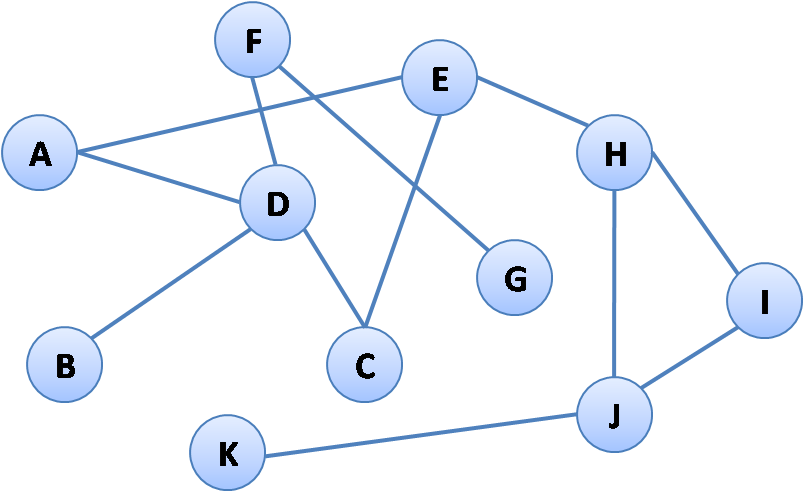
\includegraphics[width=.5\textwidth]{\img/dfsbfsgraph.png}
\end{center}

Using recursive depth-first traversal, list the vertices in the
order they are visited as we search from vertex $J$ to vertex
$G$. When we visit a vertex, we explore its outgoing edges in
alphabetical order. Do not list a vertex again if you backtrack to it.

\begin{framed}
\medskip
\answer{34em}{J, \ H, \ E, \ A, \ D, \ B, \ C, \ F, \ G}\phantom{|}
\end{framed}

List the vertices of the path found from $J$ to $G$ by the search.

\begin{framed}
\medskip
\answer{34em}{J, \ H, \ E, \ A, \ D, \ F, \ G}\phantom{|}
\end{framed}

Using a breadth-first traversal, list the vertices in the order that
they are visited as we search from vertex $J$ to vertex $G$. When we visit
a vertex, we explore its outgoing edges in alphabetical order.

\begin{framed}
\medskip
\answer{34em}{J, \ H, \ I, \ K, \ E, \ A, \ C, \ D, \ B, \ F, \ G}\phantom{|}
\end{framed}

List the vertices of the path found from $J$ to $G$ by the search.

\begin{framed}
\medskip
\answer{34em}{J, \ H, \ E, \ A, \ D, \ F, \ G}\phantom{|}
\end{framed}

\RUBRIC
Part (a)
TAGS: graph, traverse-ds

Gradescope rubric:
+0.25pt DFS Nodes: J, H, E, A, D, B, C, F, G
+0.25pt DFS Path: J, H, E, A, D, F, G
+0.25pt BFS Nodes: J, H, I, K, E, A, C, D, B, F, G
+0.25pt BFS Path: J, H, E, A, D, F, G

Commentary:
  One point per answer. Half credit for a minor mistake
  like listing D again when backtracking.

  DFS nodes: J, H, E, A, D, B, C, F, G
  DFS path: J, H, E, A, D, F, G

  BFS nodes: J, H, I, K, E, A, C, D, B, F, G
  BFS path: J, H, E, A, D, F, G
ENDRUBRIC

\part[1]\TAGS{graph}
In an undirected graph with $v$ vertices, what is the maximum possible
number of edges? (This kind of graph is called a \emph{complete
  graph}). Express your answer in closed form as a function of $v$.

\begin{framed}
\medskip
\answer{34em}{$v(v-1)/2$}\phantom{|}
\end{framed}

\enlargethispage{5ex}
A path in a graph is called a {\em simple cycle} if it lets you go
from a vertex to itself without repeating an edge or any intermediate
vertex. What is the maximum possible number of edges in a graph with
$v$ vertices that contains no simple cycles?

\begin{framed}
\medskip
\answer{34em}{$v$}\phantom{|}
\end{framed}

\RUBRIC
Part (b)
TAGS: graph

Gradescope rubric:
+0.5pt  (1st blank): EITHER -- v(v-1)/2
+0.25pt (1st blank):     OR -- O(v^2)
+0.5pt  (2nd blank): EITHER -- v-1
+0.25pt (2nd blank):     OR -- v

Commentary:
  Half points: v(v-1)/2 = (v^2-v)/2 = v choose 2
  Half of that for anything else in O(v^2)

  Half points: v-1
  Half of that: v
ENDRUBRIC

\end{parts}
